\begin{document}
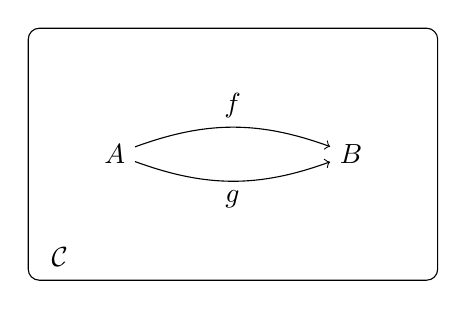
\begin{tikzpicture}
  \draw[rounded corners] (-2.6,-1.6) rectangle (2.6,1.6);
  \node at (-2.2,-1.3) {$\mathcal{C}$};
  \node (A) at (-1.5,0) {$A$};
  \node (B) at (1.5,0) {$B$};
  \draw[->] (A) to[bend left=20] node[above] {$f$} (B);
  \draw[->] (A) to[bend right=20] node[below] {$g$} (B);
\end{tikzpicture}
\end{document}
